\documentclass[11pt]{article}

\usepackage[margin=0.75in]{geometry}
\usepackage{indentfirst}
\usepackage{graphicx}
\usepackage{hyperref}
\usepackage{caption}
\usepackage{amsmath}

\bibliographystyle{siam}

\title{The generality of self-control}
\author{
  Chen, Kent\\
  \texttt{kentschen}
  \and
  Lee, Rachel\\
  \texttt{reychil}
  \and
  LeRoy, Benjamin\\
  \texttt{benjaminleroy}
  \and
  Liang, Jane\\
  \texttt{janewliang}
  \and
  Udagawa, Hiroto\\
  \texttt{hiroto-udagawa}
}



\begin{document}
\maketitle

\abstract{% tex file for abstract
\par Self-control is an interesting field of behavioral research with broad 
implications for our day-to-day experiences. Being able to appropriately 
regulate and check our impulses and reactions to various everyday stimuli 
is necessary for maintaining health and high-functionality in society. 
Thus, relating a subject’s ability to control risky behavior to an area 
of the brain has been the focus of many studies. One approach to 
capturing these neurological facets is to use functional magnetic resonance 
imaging (fMRI). Our goal is to identify active regions of the brain using 
fMRI data from a Balloon Analogue Risk Task (BART) study described in 
Cohen's \textit{The Development and Generality of Self-Control} 
\cite{CohenSelfControl}. When possible and logically sound, we will attempt 
to reproduce the data preprocessing and analysis outlined in the paper. 
However, many of our approaches deviate considerably from the methods 
used by Cohen, either out of necessity from our lack of pre-packaged 
software or when we were inspired explore other directions. Ultimately, we 
will compare the active regions identified by our analysis with those 
detected by the Cohen's paper. 
}

\section{Introduction}
	% tex file for introduction
\par This paper, \textit{The Development and Generality of Self-Control} \cite{CohenSelfControl},  and its associated fMRI studies are concerned with the relationship between impaired and normal self control as well as the similarities and differences across the brain relating to self-control. The entire paper explores multiple studies (of multiple study types), but we will just focus on the third and final study, which compares four different types of self control among healthy adults to see if they are related to each other. Very little relationship was found between these behavioral tasks, in contrast to the vast majority of existing literature, which argues for a unified notion of self-control, which is why we have decided to narrow the data analysis approaches to just the BART study. The BART study primarily focused on the inflation/deflation of a balloon that could pop; the fMRI scans show blood flow to the brain in an attempt to reveal control over risk-taking behavior while subjects participate in this particular study.
\par The rest of this report will go further in detail on the processes that we have tried to mimic from the original analysis of the data, but here is a brief overview of the work we have accomplished so far. We have looked into spatial smoothing of the data on the voxels of the brain. After realizing that there are many factors that could contribute to noise in the data, we decided it would be beneficial to look into smoothing modules in Python that could handle n-dimensional datasets to clarify which voxels are more important than other voxels. After obtaining convolved time courses for each subject, we turned to fitting simple and multiple linear regression models to each subject. Since examining the behavior of blood flow in the voxels over time was of such great interest, we also considered modeling the behavior as a time series using an autoregressive integrated moving average (ARIMA). 


\section{Data}

	% tex file for data
\par \indent The Balloon Analogue Risk Task (BART) measures risk-taking 
behavior by presenting participants with a computerized balloon. The 
participant can earn money incrementally by pumping up the balloon, but after 
an unknown threshold, the balloon will explode. At any time, the participant 
elect to cash out his or her earnings, but doing so eliminates the potential to 
gain additional money through pumps. If the balloon explodes, the participant 
loses all of the money for the trial. For this study, BART and fMRI data for 24 
subjects was collected. The mean age of the subjects was 20.8, and ten of the 
subjects were female. Four behavioral variables were recorded for each subject: 
the average number of pumps for each balloon, the average amount of money 
earned across runs, the number of exploded balloons, and the number of trials. 
There were also three model conditions: events for inflating the balloon 
(excluding the very last inflation of each trial), the last inflation before an 
explosion, and the event of cashing out (the balloon explosion was not included 
as an event). Of interest for our work is the blood-oxygen-level dependent 
(BOLD) imaging data recorded for each subject during the course of task. Each 
subject's BOLD data was recorded as 64 by 64 image matrices in 34 slices, with 
a variable number of time points. 

	
\section{Methods}
	\subsection{Smoothing}
	
		% tex file for smoothing
\par \indent Due to the random nature of human subjects and their movements, a certain extent of smoothing must be performed on the spatial dataset so that the ‘noisy’ data can be cast off from the data that represent significant changes in blood flow in the brain. By doing so, researchers and anyone else investigating the data will be able to distinguish between non-brain scans versus actual brain scans. Each voxel of the brain is represented on a measure of blood flow intensity, and so a series of steps must be taken so that it is correctly convolved to most closely and accurately depict what was happening at a certain point in the brain at a certain time. After researching quite extensively, we decided to use a convolution involving a Gaussian kernel in order to smooth the three dimensional data. Originally, we were going to try and write a smoothing function from scratch, by implementing a rudimentary rudimentary average-over-neighbors method. However, discussions with mentors lead us to the scipy module called \texttt{ndimage.filters} that has a function that performs a Gaussian filter on n-dimensional data. This was exactly what we needed so rather than reinventing the wheel, we will be smoothing the data with this module.

	\subsection{Convolution and Time Correction}

		% tex file for convolution
\subsubsection{Convolution}
\par \indent Our study is structured around event-related neurological 
stimulus, rather than block stimulus, as was the case of the data used in 
class examples. So, we could not repurpose the class approach for 
representing the hemodynamic response to our analysis. 

\par It is assumed that there is a relationship between the hemodynamic 
response to the neurological stimuli. Further, there is the assumption that 
a single stimulus generates a delayed hemodynamic response that mirrors a 
double-gamma function, and that multiple stimuli have an additive nature, as 
defined below: 

\begin{equation} \label{eq:convolve}
r(t)= \sum_{i=1}^n \psi_{i} \phi_{i}(t-t_i)
\end{equation}

\noindent where $\psi_i$ is the amplitude of the response stimulus (assumed to 
be always $1$ in our case), and $\phi_{i}$ is the hemodynamic response started 
at the $i$th stimulation ($t_i$).

\par We attempted five approaches that can each be grouped into one of three 
subcategories: \textbf{(1)} a strict replication of equation 
\ref{eq:convolve}; \textbf{(2)} a matrix multiplication equivalent to 
\textbf{(1)}; and \textbf{(3)} a complex function that takes advantage of the 
speed of \texttt{np.convolve}. This complicated function first splits the 
(two-second)intervals between each scan into a given number of even slices, 
then puts the stimulus into the closest slice with respect to time, and 
finally calls \texttt{np.convolve} on this much longer time series and a 
detailed hrf function, before reducing back down to the dimensions of the 
original scan time series at two-second intervals. Detailed exploration of 
this matter can be found in Appendix \ref{app_convolution}.

We compared these methods based on accuracy and speed. Figure 
\ref{fig:convolution_a} displays an accuracy comparison, and 
Table~\ref{fig:convolution_a} shows the accuracy based off of 
\texttt{ipython}'s \%\texttt{timeit} magic command.



\begin{figure}[ht]
\centering
	\begin{minipage}[b]{0.45\linewidth}
		\centering
		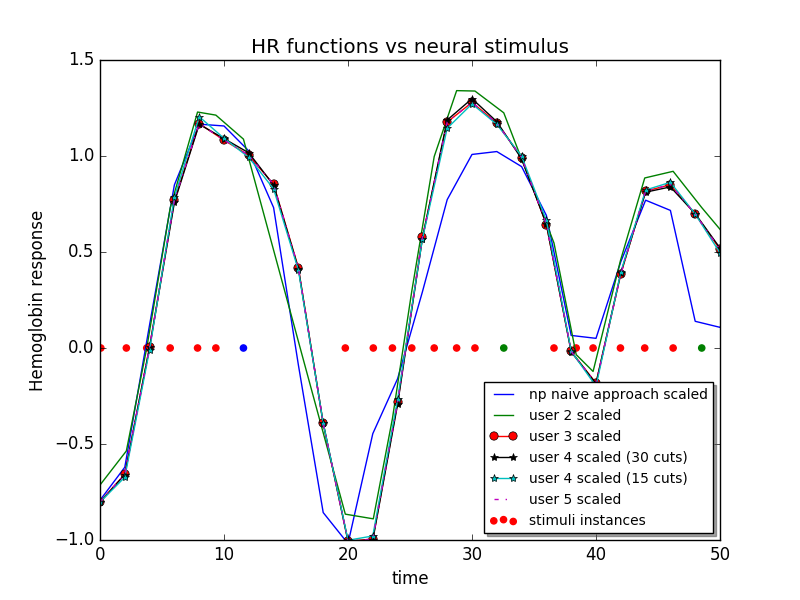
\includegraphics[width=.8\linewidth]{../images/convolution_vs_neural_stimulus}
		% needs to be from the event_related_HRF_script2.py 
		\caption{\scriptsize{Different convolution functions vs. the Neural stimulus}}
		\label{fig:convolution_a}

	\end{minipage}
\quad
	\begin{minipage}[b]{0.45\linewidth}
		\centering
		\begin{tabular}{|l | c|}
		\hline
		name in graph       & Speed per loop \\
		\hline
		np naive approach & 14.4 $\mu$s  \\
		user 2     		    & 972 ms  \\
		user 3     		    & 1.15 s    \\
		user 4 (15 cuts)      & 98.3 ms \\
		user 4 (30 cuts)      & 185 ms  \\
		user 5     	 	    & 110 ms   \\
		\hline
		\end{tabular}
		\vspace{5mm}
		\label{tab:convolution_a}
		\captionof{table}{\scriptsize{Speed to create HRF predictions for 
		Subject 001, all conditions}}
	\end{minipage}
\end{figure}

\par \noindent The first method in the table, ``np naive approach'', blindly 
plugs our data into the \texttt{np.convolve} function. It is provided to 
showcase potential speed. The failure of the "np naive approach" was the 
motivating factor behind the rest of the hemodynamic response convolution 
analysis, due to a lack of equidistant spacing of stimulus and scans. The 
``user 2'' and ``user 3'' functions runs fall under subcategory 
\textbf{(1)}. ``user 2'' was the first approach to
match the theory, but it matches the stimulation times and not the scan times.
``user 3'' is the most theoretically sound model (and is our standard for 
accuracy). The ``user 5'' falls under subcategory \textbf{(2)}, ``User 5''  is
our matrix version of the theory, and has the same accuracy as ``user 3''. The 
``user 4'' models falls under subcategory \textbf{(3)}, the methods that use the
grid cut usage of \texttt{np.convolve} with notations for the number of slices 
between each scan. We concluded that "user 4 (15 cuts)" was the best approach 
since it gives us speed and very close accuracy to the golden standard - ``user 
3".

\subsubsection{Time Correction}

\par \indent The fMRI machine scans each voxel at a slightly different time. 
In our case, the lowest horizontal slice was scanned first, with the later 
scans obtained in order progressively toward the top of the brain. The signs 
of this linear change in time of scan was observed when running simple 
regression on the data and found that the hemodyamic response $\hat{\beta}$ 
values from all conditions grouped together. We corrected for the time 
differences by shifting the times of stimuli ``backwards'' for voxels scanned 
later to directly correct for the delay of the scan (assuming that each layer 
of the scan took 2/34 of a second).

\subsubsection{Multiple Conditions}

\par \indent Originally, we used multiple regression to acount for the 
three different types of stimulus (pump, explode, cash-out) and examine if the 
separation of these stimuli can better describe the response. We did this by 
creating separate predicted hemodynamic reponses for each condition to allow 
for different amplitudes for each type of condition. As will be noted in 
Section \ref{model_selection} portion later, we did not observe a large 
difference in the results values we obtained, so we did not continue with 
this exploration. In Figure \ref{fig:all_cond_time}, we can see the different 
conditions separated the responses for each condition.
 

\begin{figure}[ht]
\centering
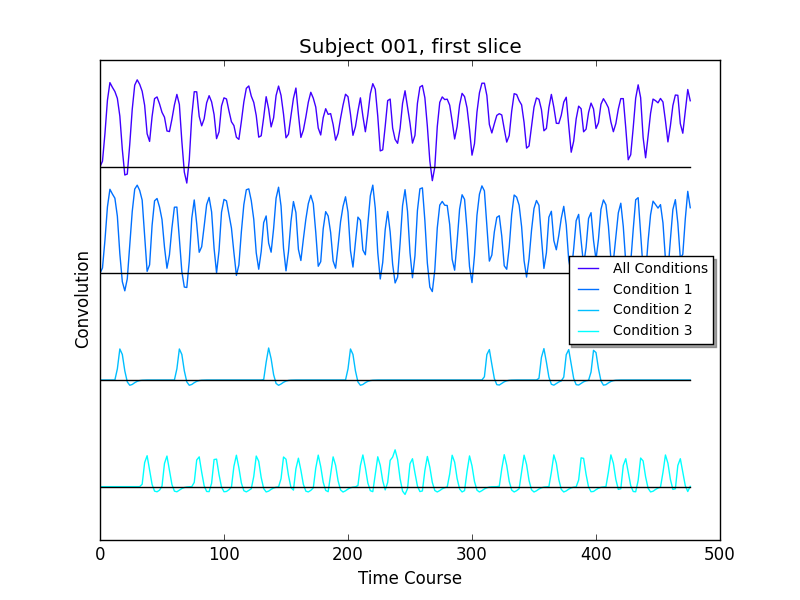
\includegraphics[scale=.5]{../images/all_cond_time}  
\caption{Plotting all predicted HR for conditions.}
\label{fig:all_cond_time}
\end{figure}

A more detailed discussion about our approach and the theory behind convolution 
of the hemodynamic response with the neurological response can be found 
in Appendix \ref{app_convolution}.


		
	\subsection{Linear Regression}
	
		% tex file for regression
		
	\subsection{Model Selection}
		
		% model comparison

\par In order to select the best set of features for our $X$ matrix, and also 
compare the use of a single condition feature vs each of the 3 different types
of conditions as 3 seperate features we decided to utilize model comparison, 
specificially AIC,BIC, and Adjusted $R^2$ metrics. Using small expressive
subset of the subjects ($002$,$003$, and $014$) we abused the metric's by
averaging across all voxels and people.  We visualized values in the Figures
\ref{fig:AIC},\ref{fig:BIC}, and \ref{fig:adjR2}, where the x axis follows the 
following structure in Table \ref{tab:plot}.

\par From these plots, you can observe that we don't gain my from adding
the conditions seperated, and from the BIC, we decided that the fourier
features didn't add enough benefit to justify the increase of features, so we'll
be using the model that includes a single HRF for all the conditions, a linear
drift feature, and the first 6 principle components.

\begin{table}
\centering
	\begin{tabular}{l ||  l   |  l  |   l    | l  | l  |  l}
X value & 1 &        2       &             3       &     4         &        5        &         6       \\
	 \hline
	 & HRF &   HRF       &  HRF            & HRF         &  HRF        & HRF  \\
	 &        &   + DRIFT &  + DRIFT      & + DRIFT  &  + DRIFT   & + DRIFT  \\
	 &        &                 &  + FOURIER &  + PCA 4 &  + PCA 6   & + FOURIER \\
	 &        &                 &                      &                &                   & +  PCA 6 \\
	

	\end{tabular}
\caption{Explaining Plot X values}
\label{tab:plot}
\end{table}


%\begin{table}
%
%\begin{minipage}[b]{1\linewidth}
%	\centering
%	\scriptsize{\begin{tabular}{l ||   l  |  l  | l  | l  |l   |  l}
%	 & HRF &   HRF     &  HRF       & HRF      &  HRF       & HRF  \\
%	 &     &   + DRIFT &  + DRIFT   & + DRIFT  &  + DRIFT   & + DRIFT  \\
%	 &     &           &  + FOURIER &  + PCA 4 &  + PCA 6   & + FOURIER \\
%	 &     &           &            &          &            & +  PCA 6 \\
%	\hline
%	All conditions together   &  589.313 &  503.388 &  452.366 & 337.296 & 288.452 &   266.126 \\
%	All conditions seperately & 587.824 &  501.184 &  449.337 &   331.995 & 286.85 &   264.756 \\
%	\end{tabular}}
%	\label{tab:AIC}
%	\center{\caption{AIC}}
%\end{minipage}	
%
%\begin{minipage}[b]{1\linewidth}
%	\centering
%	\scriptsize{\begin{tabular}{l ||   l  |  l  | l  | l  |l   |  l}
%	 & HRF &   HRF     &  HRF       & HRF      &  HRF       & HRF  \\
%	 &     &   + DRIFT &  + DRIFT   & + DRIFT  &  + DRIFT   & + DRIFT  \\
%	 &     &           &  + FOURIER &  + PCA 4 &  + PCA 6   & + FOURIER \\
%	 &     &           &            &          &            & +  PCA 6 \\
%	\hline
%	All conditions together    &  596.409 &  514.032 &  477.202 &    365.68 &316.835&  308.702\\
%	All conditions seperately & 602.016 &  518.924 &  481.269  360.379 & &  322.33 & 314.427 \\
%	\end{tabular}}
%	\label{tab:BIC}
%	\caption{BIC}
%\end{minipage}	
%
%
%\begin{minipage}[b]{1\linewidth}
%	\centering
%	\scriptsize{\begin{tabular}{l ||   l  |  l  | l  | l  |l   |  l}
%	 & HRF &   HRF     &  HRF       & HRF      &  HRF       & HRF  \\
%	 &     &   + DRIFT &  + DRIFT   & + DRIFT  &  + DRIFT   & + DRIFT  \\
%	 &     &           &  + FOURIER &  + PCA 4 &  + PCA 6   & + FOURIER \\
%	 &     &           &            &          &            & +  PCA 6 \\
%	\hline
%	All conditions together    & 0.007  &  0.198  &  0.323  &  0.527   &  0.596  & 0.631 \\
%	All conditions seperately & 0.02   &  0.211  &  0.337  &    0.536  & 0.601  & 0.635\\
%	\end{tabular}}
%	\label{tab:adjR2}
%	\caption{Adjusted $R^2$}
%\end{minipage}
%
%\end{table}



\begin{figure}
\centering
	\begin{minipage}[b]{0.33\linewidth}
		\centering
		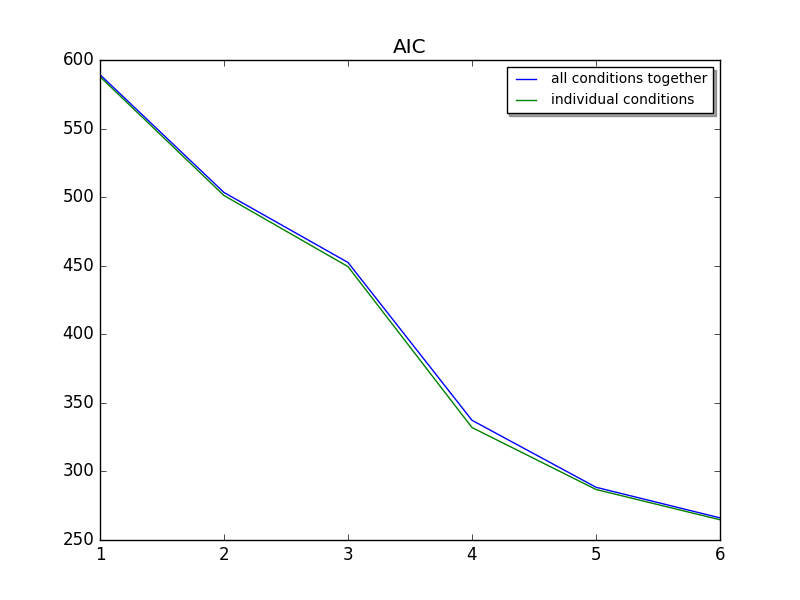
\includegraphics[width=.8\linewidth]{images/aic_better}  

		\caption{AIC}
		\label{fig:AIC}

	\end{minipage}
	\quad
	\begin{minipage}[b]{0.33\linewidth}
		\centering
		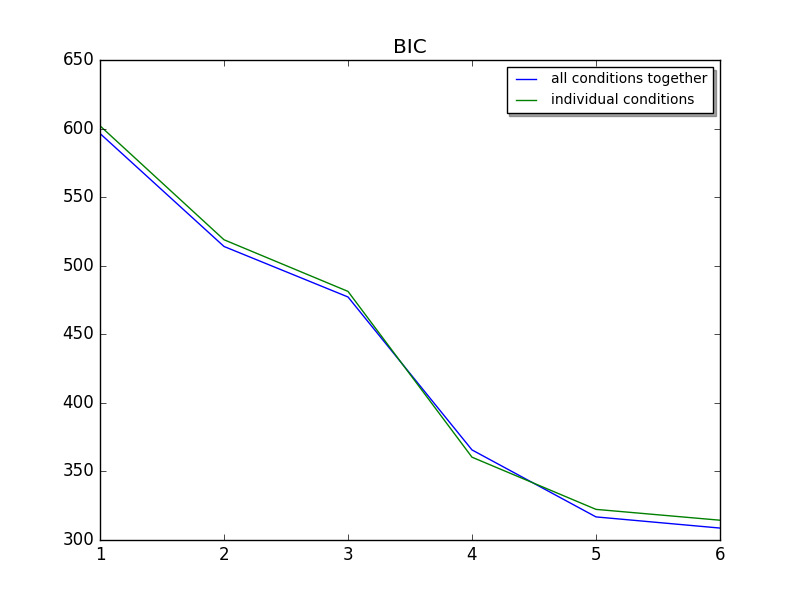
\includegraphics[width=.8\linewidth]{images/bic_better}  
		\caption{BIC}
		\label{fig:BIC}

	\end{minipage}
		
	\begin{minipage}[b]{0.33\linewidth}
		\centering
		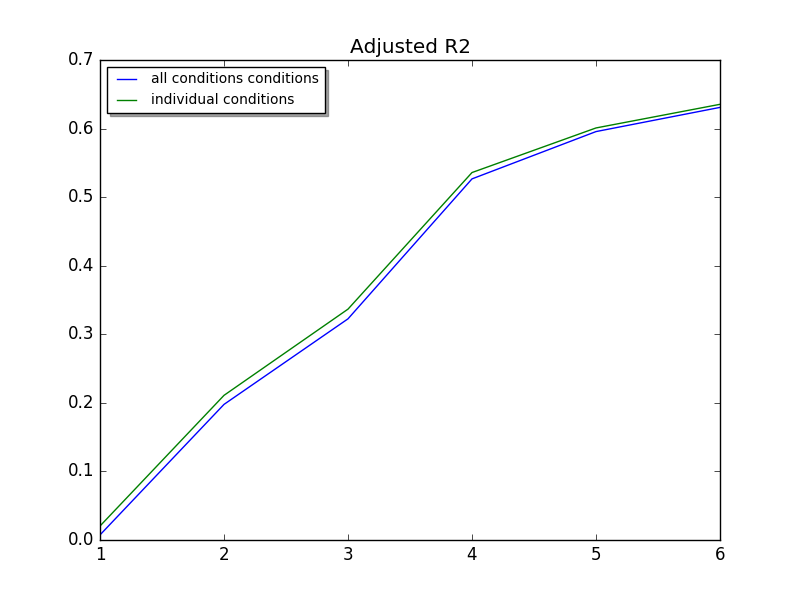
\includegraphics[width=.8\linewidth]{images/adjr2_better}  
		\caption{Adjusted $R^2$}
		\label{fig:adjr2}

	\end{minipage}

\end{figure}

	
	

	\subsection{Normality Assumptions}
	
		% tex file for normality
\par \indent The validity of our hypothesis tests for the estimated 
$\hat{\beta}$ values from the chosen linear regression model are largely 
dependent on whether we can reasonably assume that the errors in our model 
are independent and identically distributed from some normal distribution 
with mean zero and constant variance. We focus here on checking the normality 
assumption. It is generally wise to use visualizations, such as residual vs. 
fitted values plots and quantile-quantile plots to inspect residuals for 
patterns and abnormalities. However, considering the sheer quantity of data 
we are working with --- each of the 24 subjects has 64 $\times$ 64 $\times$ 34 
voxels that can each in turn be fitted to a model --- visual inspection is 
not practical. 

For this reason, we used the Shapiro-Wilk test for normality, 
which tests the null hypothesis that the data in question is normally 
distributed. A Shapiro-Wilk test was performed for each set of residuals 
corresponding to a single voxel's time course. That is, each test used around 
200 observations, or the number of time points for that particular subject. 
200 observations is not an especially large sample size, and for this reason, 
we express some concern because normality tests have low power for small 
sample sizes. Shapiro-Wilk may incorrectly fail to reject the null hypothesis 
due to this bias \cite{ghasemi2012normality}. 

The average proportion of Shaprio-Wilk test ``p-values'' above 0.05 was 0.742 
for the unmasked residuals across both subjects and voxels and noticeably 
lower at 0.630 for the masked residuals. However, since using the masked data 
is more theoretically justifiable (the unmasked data contains many voxels 
outside of the brain), we use the masked data for our analysis despite the 
lower proportion of voxels whose residuals meet our normality check. Note that 
these proportions suggest that only about two-thirds of the masked voxels have 
residuals that are approximately normal, and that the others deviate 
significantly from the normal distribution (especially when considering our 
concerns about the power of Shaprio-Wilk tests for small sample sizes). So when 
discussing our models and especially when looking at the conclusions made by 
our hypothesis tests, one should exercise caution about the validity of those 
conjectures. 

Figures \ref{fig:sw} and \ref{fig:sw_masked} compare the spatial distribution 
of the Shapiro-Wilk ``p-values'' for Subject 10's masked and unmasked data. 
The unmasked figure is very difficult to interpret, but the masked figure does 
suggest that while the spatial distribution of voxels with approximately 
normal residuals is reasonably uniform in many regions, there are a few areas 
that consistently have very low ``p-values'' at around or below the 0.05 
threshold. Examples of these regions for Subject 10 include a small area 
between the front and center of the brain and a few spots near the sides. 
However, these observations are not consistent across all subjects, so much 
of it may simply be due to noise. 

\begin{figure}[ht]
\centering
\begin{minipage}[b]{0.45\linewidth}
	\centering
	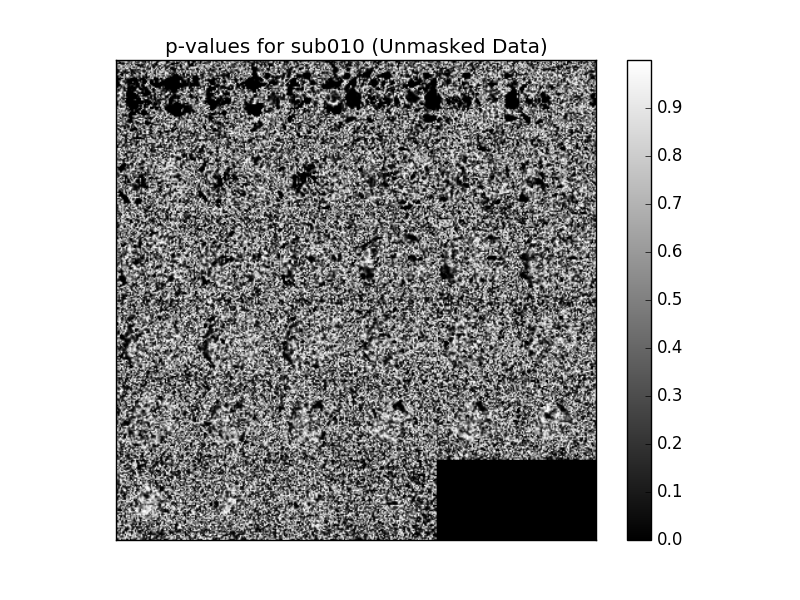
\includegraphics[width=.8\linewidth]{../images/sub010sw.png} 
	\caption{Subject 10's brain slices, with voxels colored by the magnitude of the
``p-value'' in the corresponding Shapiro-Wilk test for normality.Using unmasked residuals.}
\label{fig:sw}
\end{minipage}	
\quad
\begin{minipage}[b]{0.45\linewidth}
	\centering
		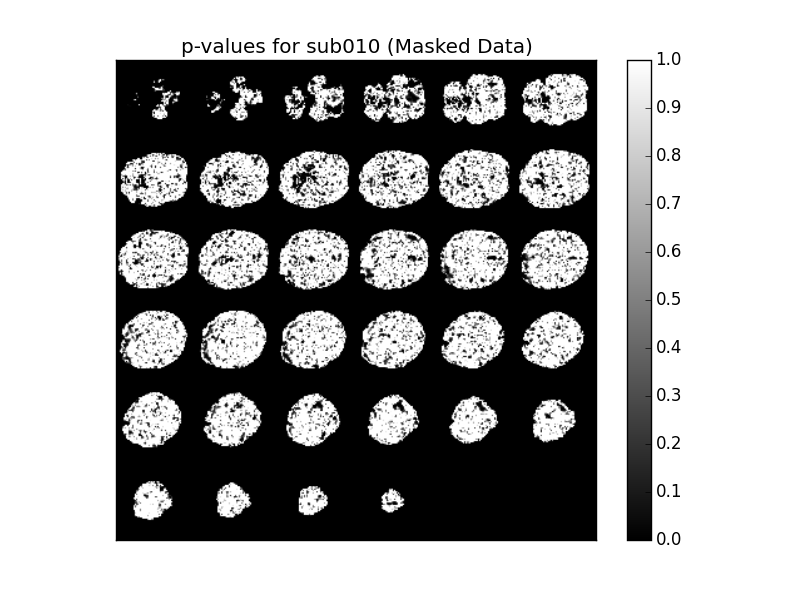
\includegraphics[width=.8\linewidth]{../images/sub010swmasked.png} 
	\caption{Subject 10's brain slices, with voxels colored by the magnitude of the
``p-value'' in the corresponding Shapiro-Wilk test for normality. Using masked residuals.}
\label{fig:sw_masked}
\end{minipage}
\end{figure}

		
	\subsection{Hypothesis Testing}
	
		% tex file for hypothesis 
\par \indent Our simple linear regression model was created to better 
understand the relationship between the voxels in a given subject's brain and 
the convolved time course. In order to measure the strength of the association 
between these two measurements, we ran a hypothesis test on the coefficients of 
the simple linear regression model for each subject. 

\par There is an individual linear model associated with each voxel in a
subject’s image (and a total of $64 \times 64 \times 34$ voxels per subject).
Thus we ran a t-test on each voxel's $\beta$ coefficient that is associated
with the HRF response. The null hypothesis for each test was that $ \beta = 0$,
with the alternative hypothesis that $\beta \neq 0$. Once we had obtained each
t-statistic, we compared this value across voxels in two ways. First, we simply
compared this t-values with voxels within a subject. In this case, we took into
account the sign of the t-statistic in our analysis. Second, we converted this
t-statistic to a "p-value", in which case the sign of the t-value will become
irrelevant and we compared across voxels without taking into account this sign.
Later, we also run a multiple comparison test using a Benjamini\–Hochberg in
order to find the voxels that are most significant.


\par Having implemented a method to compare the voxels within a single subject, 
we next examined our results for the same voxels across subjects. Our initial 
approach was to aggregate the t-statistic data between all subjects for each 
voxel. This allowed us to decrease the variability of the fit on each voxel and 
detect a more clear signal. 

\par In order to do this, we ran the hypothesis test as stated above on all 24 
subjects of the study. Then for each voxel, we took the average of the t-
statistics across the subjects. An issue with our data was the presence of 
empty space detected by the scanner that is not directly part of the brain. To 
account for this, we took the masked data of the brain and ``cut out'' the parts 
of the images that were not relevant to our analysis. Ultimately, we were left with 
a single 3-d image with each voxel representing the average t-statistics across 
all subjects in the study. This image will later be used in our clustering step in 
order to pinpoint the regions of the brain that have the strongest relationship 
with the convolved time course. 


	\subsection{Benjamini-Hochberg Correction}
	
		% tex file for Benjamini-Hochberg


	\subsection{Clustering}
	
		% tex file for clustering 
\par Now that we have the across subject average t-values for every voxel in
the brain, we are left with a 3d array of t-values that contain both negative
and positive values. Instead of manually observing patterns in these images, we
instead impelmented a clustering algorithm to split the entire 3d images into
clusters based on the voxels' relative location to each other as well as the
t-value.

\par In order to find a proper clustering algorithm, we decided to treat this
problem like a grayscale image segmentation problem and implemented a
agglomerative hierarchical cluster using Ward's method. Agglomerative means
that the clusters are built bottom up which each observation starting as its
own cluster and pairs being moved up the hierarchy. Ward's method creates
clusters based on a minimum variance criterion that miniizes the total
within-cluster variances. An example of this implimentation for a 2d image is
seen here: 
\url{http://scikit-learn.org/stable/auto_examples/cluster/plot_lena_ward_segment
 ation.html}.

In our implimentation, we defined a structure to our data using a connectivity
graph in order to ensure that each cluster is spatially constrained. Also,
since our scenario uses a 3d image, the connectivity graph will also have to
take into account this extra dimension.

\par Ultimately, the goal of this clustering is to have a better understanding
of which parts of the brain are related to the signal based on its t-values.
Once we obtain our clusters, we will both measure the within-cluster mean of
t-values as well measure the centroids of the clusters. By doing this, we hope
to see the parts of the brain that have the strongest relationship with the
signal and compare them to the results of the origin alresearch paper.




		
\section{Results}
		
	\subsection{Linear Regression Results}
	
		% tex file for regression results
\par To develop linear models, we looked at the HR from the neural response 
as a single feature and used multiple regression to take into account the 3 
different types of stimulus (pump, explode, cash-out) to see if the 
separation of these stimuli can better describe the response. Specifically, 
this allows for the prediction of different amplitudes for each type of 
stimulus's HR function in linear regression. The predictive power of these 
models was not very good [Figure \ref{fig:fit_vs_act}, \ref{fig:fit_vs_res}, 
\ref{fig:all_cond_time}]. This figures utilize the smoothed data.
  
\begin{figure}[ht]
\centering
\begin{minipage}[b]{0.45\linewidth}
	\centering
	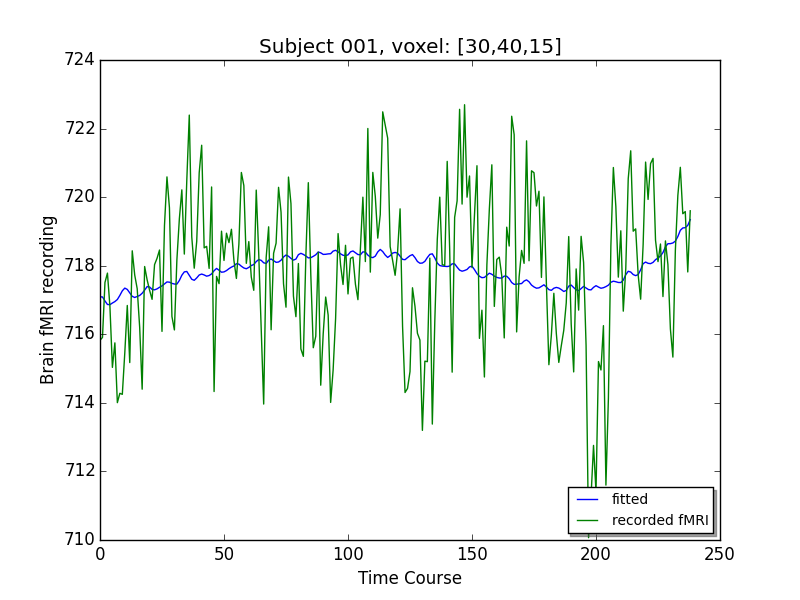
\includegraphics[width=.8\linewidth]{images/Fitted_v_Actual.png} 
	\caption{Fitted vs Actual}
	\label{fig:fit_vs_act}
\end{minipage}	
\quad
\begin{minipage}[b]{0.45\linewidth}
	\centering
		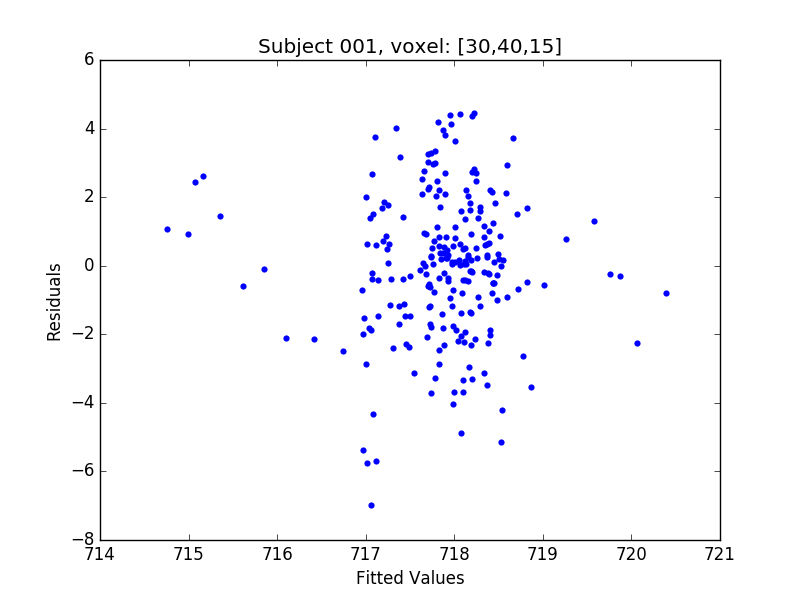
\includegraphics[width=.8\linewidth]{images/Fitted_v_Residuals.png} 
	\caption{Fitted vs Residual}
	\label{fig:fit_vs_res}
\end{minipage}
\end{figure}




\begin{figure}[ht]
\centering
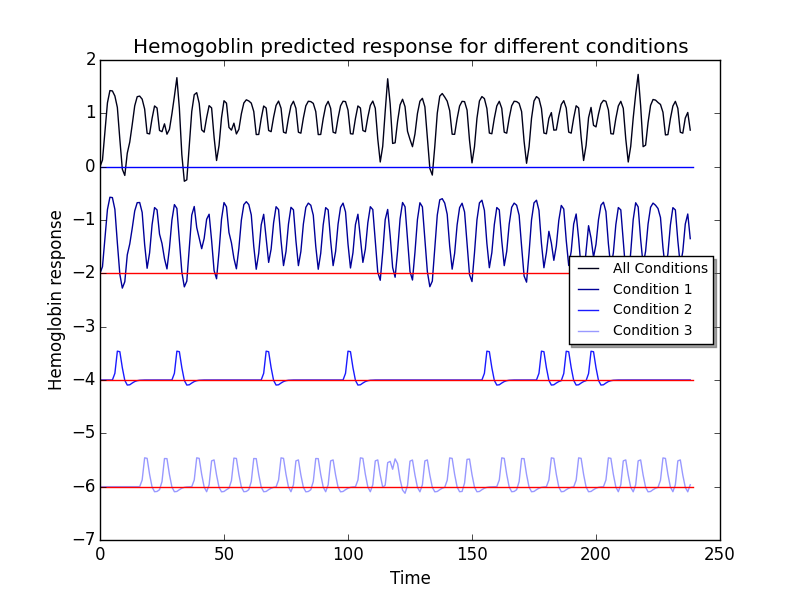
\includegraphics[scale=.5]{images/all_cond_time}  
\caption{Plotting all predicted HR for conditions.}
\label{fig:all_cond_time}
\end{figure}

As we also obtained $\hat{\beta}$ values (coefficients) from the linear 
regression models, we looked at the 3-dimensional reports of the 
$\hat{\beta}$ values, a less rigorous analysis than hypothesis testing with 
t-statistics [Figure \ref{fig:con1_beta_brain}]. 

\begin{figure}[ht]
\centering
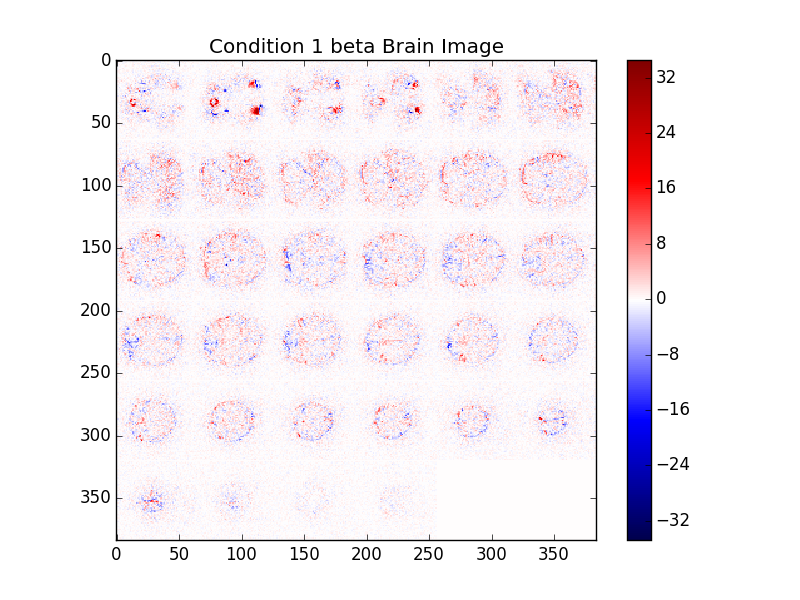
\includegraphics[scale=.5]{images/mr_cond1_beta_brain}    
\caption{$\hat{\beta}$ values for condition 1, subject 001.}
\label{fig:con1_beta_brain}
\end{figure}

The numerous other multiple regression models discussed in 
\textit{Linear Regression} should be analyzed similarly in the future. 

				
	\subsection{Hypothesis Testing Results}
	
		% tex file for hypothesis testing results
		
	\subsection{Clustering Results}
	
		% tex file for clustering results




% \begin{figure}[ht]
% \centering
% 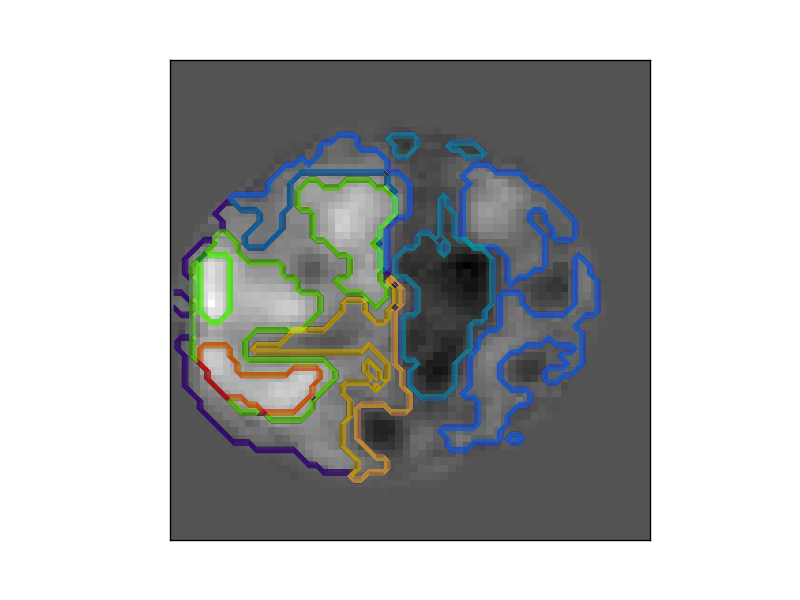
\includegraphics[scale=0.5]{images/clustering1}
% \caption{Ward clustering one slice.}
% \label{fig:mask}
% \end{figure}



\section{Discussion}
	
	\subsection{Discussion of Results}
		
		% tex file for discussion
\par \indent While very much still a work in progress, our analysis thus far 
includes methods for both data processing and modeling voxel time courses. 
Prior to doing any serious analysis, we had to smooth the data spatially for 
each subject. We also generated a reasonable convolved time course with time 
shift corrections, based on event-related neurological stimuli with 
non-constant intervals. 

\par A basic but nevertheless important model to consider is linear regression. 
We implemented both simple and multiple regression models at the individual 
subject level. In addition to the convolved time course, our multiple linear 
regression models attempt to account for more of the noise in our data by 
including terms for event conditions, linear drift, and discrete cosine 
transforms. We then checked the assumptions for the fitted models and performed 
hypothesis testing on the resulting coefficients for each voxel. Though the 
linear regression models were designed to handle each voxel for each subject's 
data individually, we aggregated the data across the 24 subjects by taking the 
means of the t-statistics corresponding to each voxel. However, one major concern 
for hypothesis testing is the issue of multiple comparisons, which we attempted to 
address using the Benjamini-Hochberg procedure. Finally, we used k-means 
clustering to further identify areas of the brain with high neurological activity 
during the events of the BART study. 




		
	\subsection{Discussion of Future Work}
	
		% tex file for future discussion
\par \indent The implementation of permutation tests, which have few 
assumptions and are easy to interpret (but computationally intensive), 
would have been useful for testing the significance of the estimated 
coefficients from linear modeling. This can serve as an alternative to 
t-tests, which make several assumptsion about the data structure. 
Somewhat relatedly, additional tests and checks for model assumptions would 
also be valuable for assessing the appropriateness of our existing hypothesis 
testing. 

\par One major issue that we were unable to fully address is how to 
appropriately aggregate the results from individual subjects to make more 
general conclusions about activation regions, as opposed to the 
activation region of a particular subject. Much of this is due to the 
considerable variety in brain positioning and shape observed between different 
subjects; there is really no such thing as an ``average'' subject. One 
approach that we tried was to simply average across subjects the binary 
t-statistic masks from the quantile-based clustering (Figure \ref{fig:avgt}). 
The result was a single ``average'' brain, but since there is considerable 
variance in brain size, shape, and so on, the justification for this method 
was not theoretically sound. Nevertheless, having that single average brain 
makes interpretation easier. For our situation, this method was able to tease 
out the high activity in the back of the brain, but not elsewhere. 

\begin{figure}[ht]
\centering
	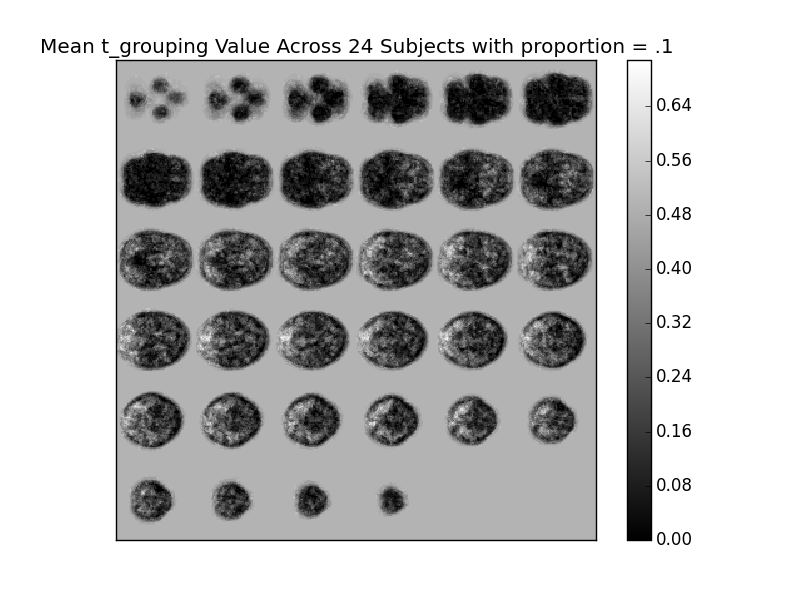
\includegraphics[width=.8\linewidth]{../images/tgroup_mean_final.png} 
	\caption{Slices from averaging the binary t-statistic masks across 
subjects. Colors indicate the proportion of subjects that identified a voxel 
as significant.}
	\label{fig:avgt}
\end{figure}

\par Additional future work could also be concerned with reproducing our 
approach for identifying actived regions on the pre-cleaned version of the 
study's data provided by the organizers of the OpenfMRI project. Those results 
could then be compared with the results from using our own pre-processing 
techniques. Since fMRI data is notoriously noisy, the different decisions made 
when cleaning the data to seperate the signal from the noise can greatly alter 
the results. So while ideally, both our pre-processed data and the 
alternatively pre-processed data would identify the same active regions, we 
acknowledge that there is a reasonably high chance that this would not be the 
case. 

\par Relating back to the issue of aggregating subjects, one great advantage 
to using the cleaned data from Ross Poldrack and the OpenfMRI project is that 
the subjects were registrated to a standard MNI anatomical template. Averaging 
clustering results across subjects would make more sense here, since the 
standard template should account for many of the differences in brain shape 
and positioning in the fMRI scanner. Near the end of our project we attempted
to incorporate the new data, but with 8 $\times$ as much data per subject and 
the nonlinear order of growths caused problems in the short term.

		

\bibliography{project}

\section{Appendix}

\begin{enumerate}
	\item Outlier Removal

	\item Convolution Analysis

	\item Smoothing

	\item Clustering (not written yet)

	\item Time Series Analysis

\end{enumerate}

\end{document}
